\section{Groups}
\label{acp-groups}

Die Gruppenseite erlaubt es, neue Rabattgruppen zu erstellen, existente zu bearbeiten und nicht mehr benötigte zu löschen. In der Suchleiste kann nach Gruppennamen gefiltert werden.

\begin{figure}[ht]
    \centering
    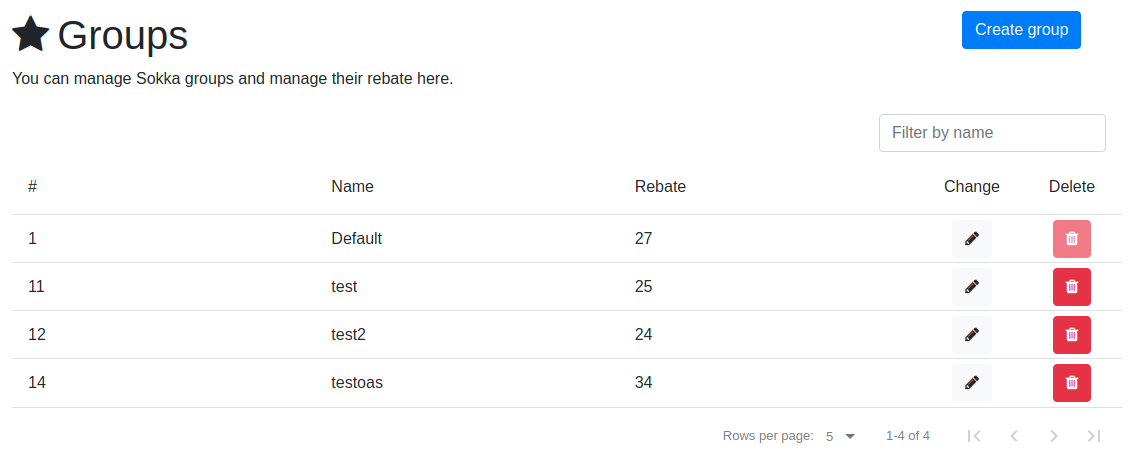
\includegraphics[width=0.8\textwidth]{images/ACP/groups.png}
    \caption{Die Gruppenseite des Sokka-ACPs}
\end{figure}

Wenn man für eine bestimmte Gruppe von Nutzern einen allgemein gültigen Rabatt für Bestellungen von Menüs sowie Produkten hinterlegen möchte, so kann man für diese Nutzer mit einem Klick auf den \glqq Create group\grqq -Button eine Rabattgruppe erstellen.

Alle Rabattgruppen, außer die Default-Gruppe, sind löschbar. Der Name und der Rabatt der Gruppe kann über den \glqq Change\grqq -Button via Slider angepasst werden.

\begin{figure}[ht]
    \centering
    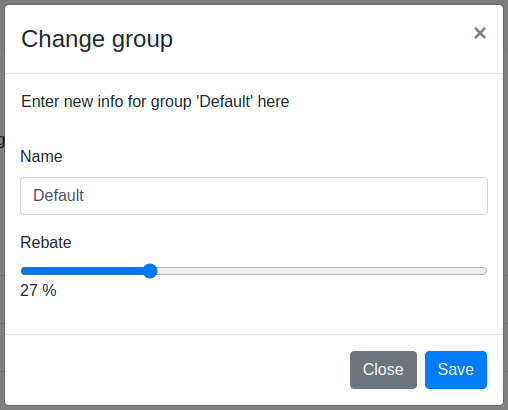
\includegraphics[width=0.6\textwidth]{images/ACP/groups_modal.png}
    \caption{Der Dialog zum Ändern des Rabatts von Rabattgruppen im Sokka-ACP}
\end{figure}